% !TEX root = report.tex

\section{Processing Pipeline}
\label{sec:processing_architecture}

High level descripion of the processing flow:

Throughout the report: extract Spectrograms, classify image.

\section{Signals and Features}
\label{sec:model}

\subsection{Google Dataset}

% Measurement setup, data preprocess (describe the google dataset)

The Speech Commands datasets, described in \cite{warden2018speech}, provides
thousands of one second recording of $35$ differen words. The recordings are
mainly of volounteers, who used their own device to record the words in a
closed room wherever they happened to be (not in a studio setting).
Ideally each volounteer only recorded the $135$ requested utterances once, so the
dataset provides good variability of voices.
The utterances have a duration of one second.
To more precisely align the recorded clips, the audio was acquired for $1.5$
seconds and the $1$ second clip that contained the highest overrall volume was
extracted.
Several background noise recording are included as well.
The full dataset includes $105829$ utterances of $35$ words, saved in
\textit{.wav} format at $16$ KHz rate.
The dataset is released under the Creative Commons BY $4.0$ License \cite{ccby4}.

The dataset ships with a function to split the data in train, validation and
test folds, as well as two example lists of validation data ($9981$ utterances)
and test data ($11005$ utterances).
Throughout the experiments, those lists were used.
% both for the practicality of having them ready, but also to keep with the
% spirit of the dataset as a tool to enable meaningf

\subsection{Mel spectrogram and Mel-frequency Cepstral Coefficients}

The audio data in the dataset is available as a vector of amplitudes over time,
sampled at $16$ KHz. In this representation, the classification task is quite
hard.
The Fourier transform allows to convert a signal from the time domain into the
frequency domain. The result is called spectrum of the signal. This transform
is efficiently computed using the Fast Fourier Transform algorithm.

The short-time Fourier transform accounts for variations of the content of an
audio signal over time. Instead of computing the FFT of the entire signal, the
FFT is computed on overlapping windowed segments of the signal: each window has
length \texttt{n\_fft} and the next window is extracted after
\texttt{hop\_length} samples.
The results of the FFT in each window are stacked to obtain the spectrogram.

The human ear does not perceive frequencies on a linear scale: the difference
between $200$ and $400$ Hz is very marked, whereas two notes at $8000$ and
$8200$ Hz are almost indistinguishable. The mel scale, proposed by Stevens,
Volkmann, and Newmann \cite{melscale1937}, introduces a unit of pitch built in
such a way that equal distances on the scale sound equally distant to the human
listener.
The mel spectrogram is a spectrogram where the frequencies are converted to the
mel scale. To do so, a Mel spaced filterbank is generated (a 10 filters version
is shown in \fig{fig:mel10_filterbank}) and the FFT results are multiplied with
a dot product with each filter, obtaining \texttt{n\_mel} values for each
timestep.

\begin{figure}[t!]
    \centering
    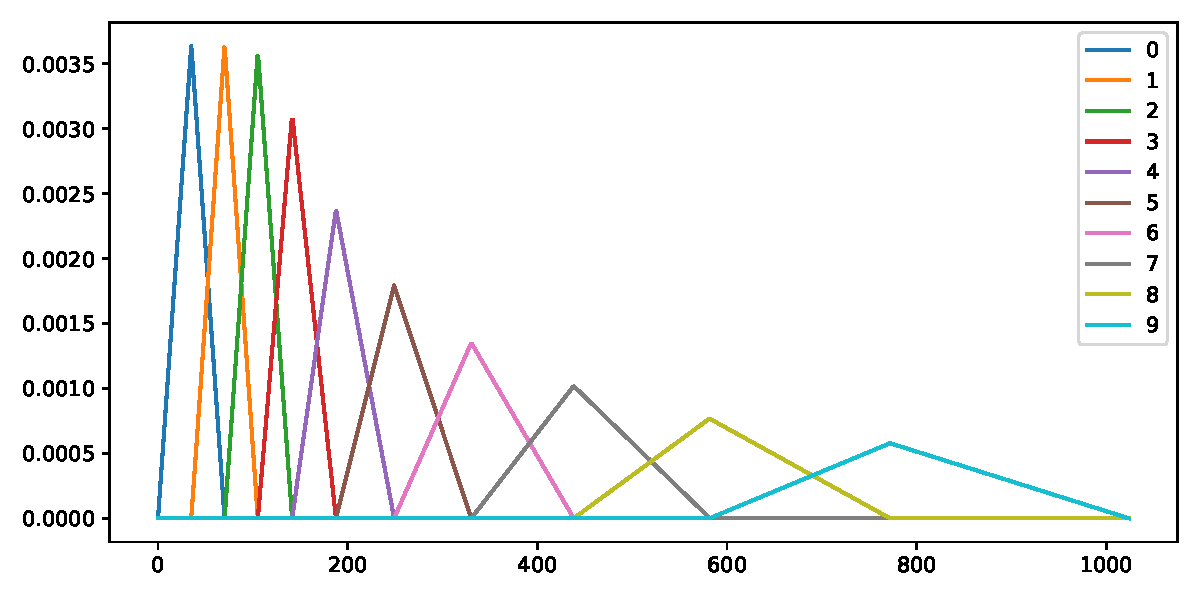
\includegraphics[width=0.8\linewidth]{mel10_filterbank.pdf}
    \caption{An example of a 10 filters Mel filterbank}
    \label{fig:mel10_filterbank}
\end{figure}

The resulting coefficients are highly correlated: the Discrete Cosine Transform
can be applied to decorrelate the filter bank coefficients and obtain a
compressed representation.
The results are the Mel-frequency Cepstral Coefficients.

The spectrograms were obtained using the \texttt{librosa} library \cite{brian_mcfee_2020_3955228}.
The values used to generate the mel spectrograms are listed in
\tab{tab:mel_values}.
The values used to generate the mel frequency cepstral coefficients are listed
in \tab{tab:mfcc_values}.
An example waveform for the word ``happy'' and the relative spectrograms are
shown in \fig{fig:happy_specs}.

\begin{figure}[t!]
    \centering
    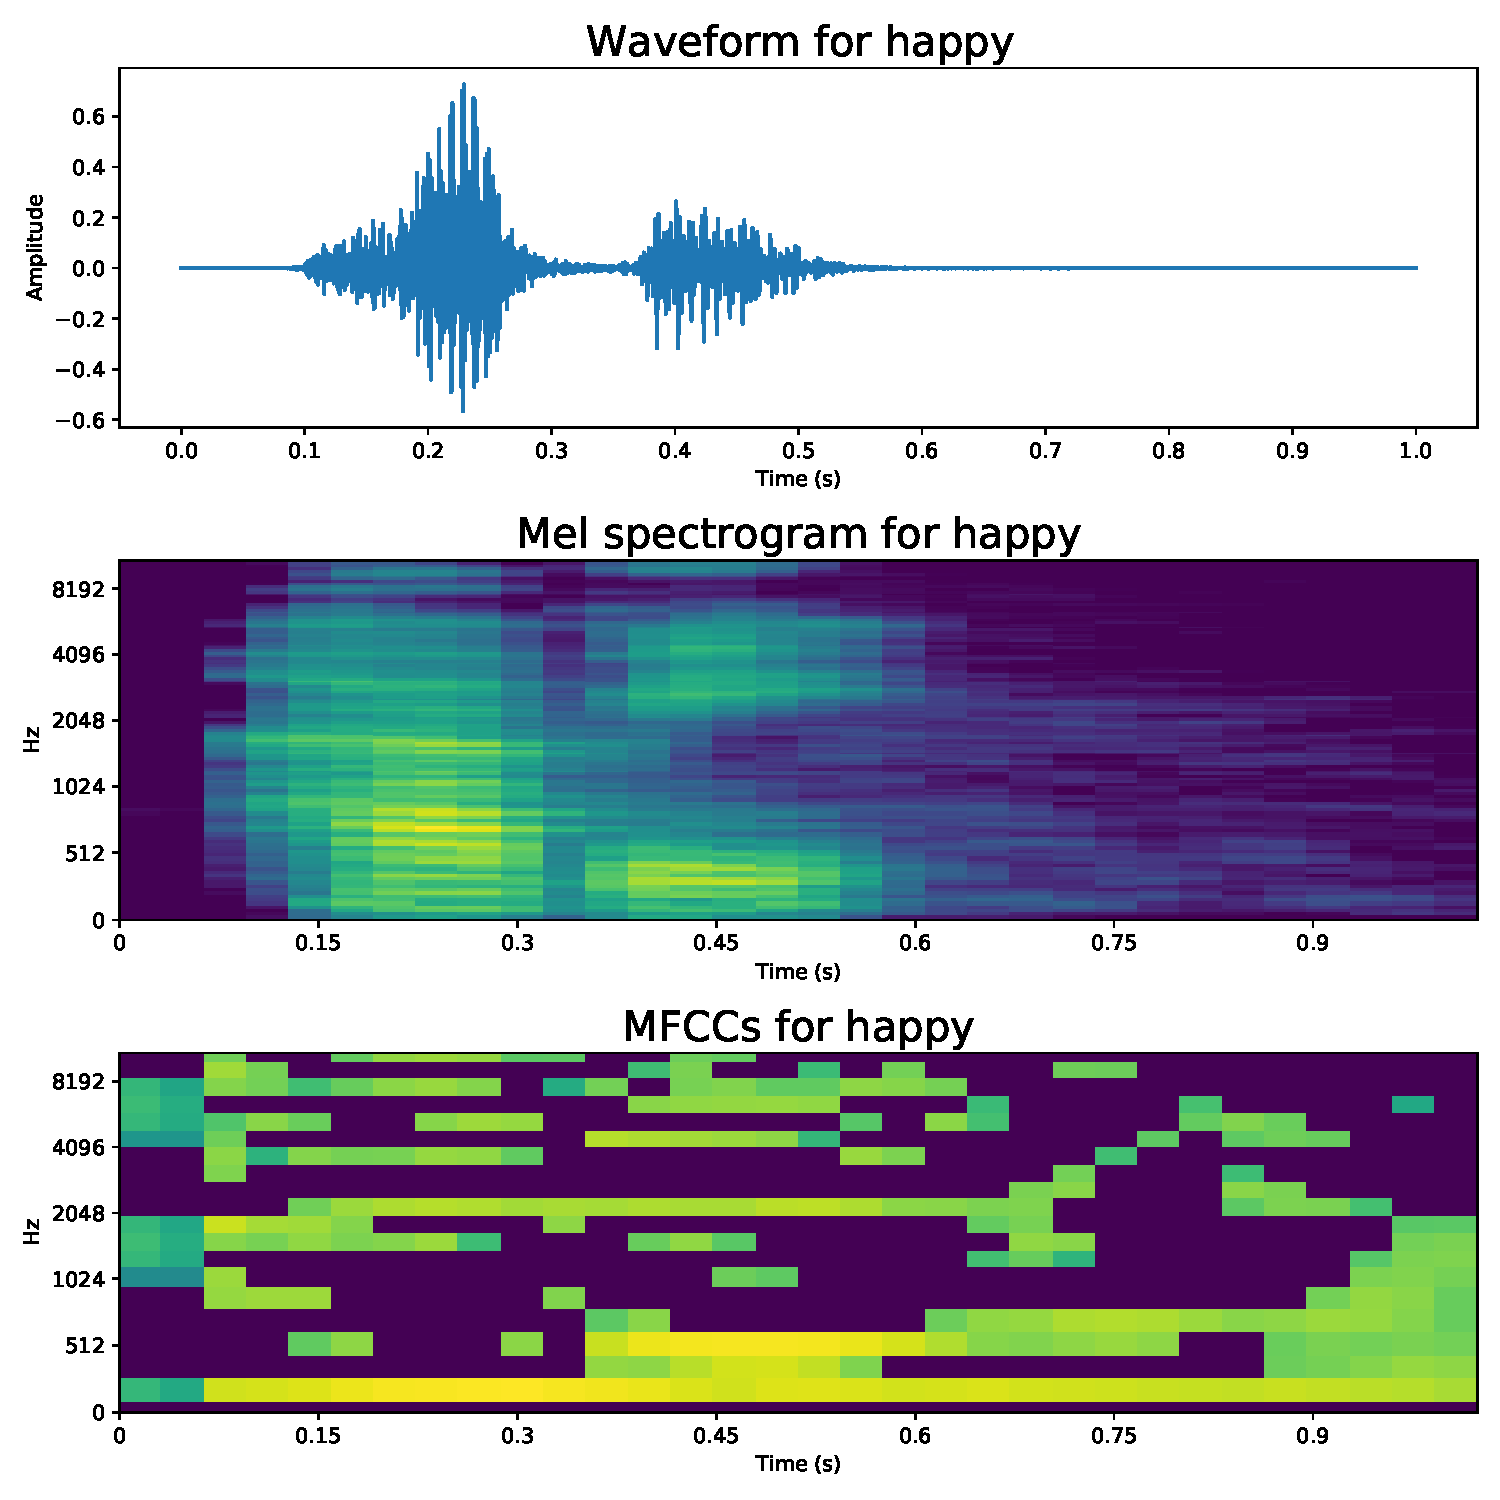
\includegraphics[width=0.8\linewidth]{happy_specs.pdf}
    \caption{
    Waveform and spectrograms for the word happy. Note that the y axis of the
spectrograms are labeled as Hz, but this is only to read more easily the plot
and understand to which frequencies the important bins correspond to. }%
    \label{fig:happy_specs}
\end{figure}

\begin{table}[t!]
    \centering
    \caption{
    Values used to generate the mel spectrograms. The dataset ``mela1'' also
has the parameter \texttt{fmin}$=40$.}
    \label{tab:mel_values}
    \begin{tabular}{|c|cccc|}
        \hline
        % name & \texttt{n\_mel} & \texttt{n\_fft} & \texttt{hop\_length} & shape \\
        name & n\_mel & n\_fft & hop\_length & shape \\
        \hline
        mel01 & 128 & 2048 & 512   & (128, 32) \\
        mel02 & 64  & 4096 & 1024  & (64, 16) \\
        mel03 & 64  & 2048 & 512   & (64, 32) \\
        mel04 & 64  & 1024 & 256   & (64, 64) \\
        mel05 & 128 & 1024 & 128   & (128, 128) \\
        mel06 & 128 & 1024 & 256   & (128, 64) \\
        mel07 & 128 & 2048 & 256   & (128, 64) \\
        mel08 & 128 & 512  & 256   & (128, 64) \\
        mel09 & 128 & 512  & 128   & (128, 128) \\
        mel10 & 128 & 2048 & 128   & (128, 128) \\
        mel11 & 128 & 256  & 128   & (128, 128) \\
        mel12 & 128 & 4096 & 256   & (128, 64) \\
        mel13 & 128 & 512  & 256   & (128, 64) \\
        mel14 & 128 & 256  & 256   & (128, 64) \\
        mel15 & 128 & 3072 & 256   & (128, 64) \\
        mela1 & 80  & 1024 & 128   & (80, 128) \\
        \hline
    \end{tabular}
\end{table}

\begin{table}[t!]
    \centering
    \caption{Values used to generate the MFCC spectrograms}
    \label{tab:mfcc_values}
    \begin{tabular}{|c|cccc|}
        \hline
        % name & \texttt{n\_mfcc} & \texttt{n\_fft} & \texttt{hop\_length} & shape \\
        name & n\_mfcc & n\_fft & hop\_length & shape \\
        \hline
        mfcc01 & 20  & 2048 & 512  & (20, 32) \\
        mfcc02 & 40  & 2048 & 512  & (40, 32) \\
        mfcc03 & 40  & 2048 & 256  & (40, 64) \\
        mfcc04 & 80  & 1024 & 128  & (80, 128) \\
        mfcc05 & 10  & 4096 & 1024 & (10, 16) \\
        mfcc06 & 128 & 1024 & 128  & (128, 128) \\
        mfcc07 & 128 & 512  & 128  & (128, 128) \\
        mfcc08 & 128 & 2048 & 128  & (128, 128) \\
        \hline
    \end{tabular}
\end{table}

\subsection{Data augmentation}

Data augmentation is a technique to increase the amount of data available by
applying random, but meaningful, transformations to the data. This leads to a
noisier dataset, that should make the trained model more robust and less prone
to overfitting. The data was augmented both by modifying the waveform and the
spectrograms. An option to include the originals in the augmente dataset is
available.

\subsubsection{Time shift}

The waveform is shifted by a random amount of samples, controlled by the
parameter \texttt{max\_time\_shift}.

\subsubsection{Time stretch}

The waveform is stretched, making the sound slower or faster, controlled by the
parameter \texttt{stretch\_rate}.

\subsubsection{Spectrogram warp}

The spectrogram is warped using the \texttt{sparse\_image\_warp} function
available as a tensorflow addon.
A sequence of source landmarks is randomly selected within the image, and the
points are shifted by a random amount along both time and frequency axis. The
warp is controlled by the parameters \texttt{num\_landmarks},
\texttt{max\_warp\_time} and \texttt{max\_warp\_freq}.
The effect of warping an image is shown in \fig{fig:warp_grid}.

Several augmentations were performed, mostly focussing on the spectrogram
warping, along one or both time and frequency axis.
Values used to augment the dataset are listed in \tab{tab:aug_values}.

\begin{figure}[t!]
    \centering
    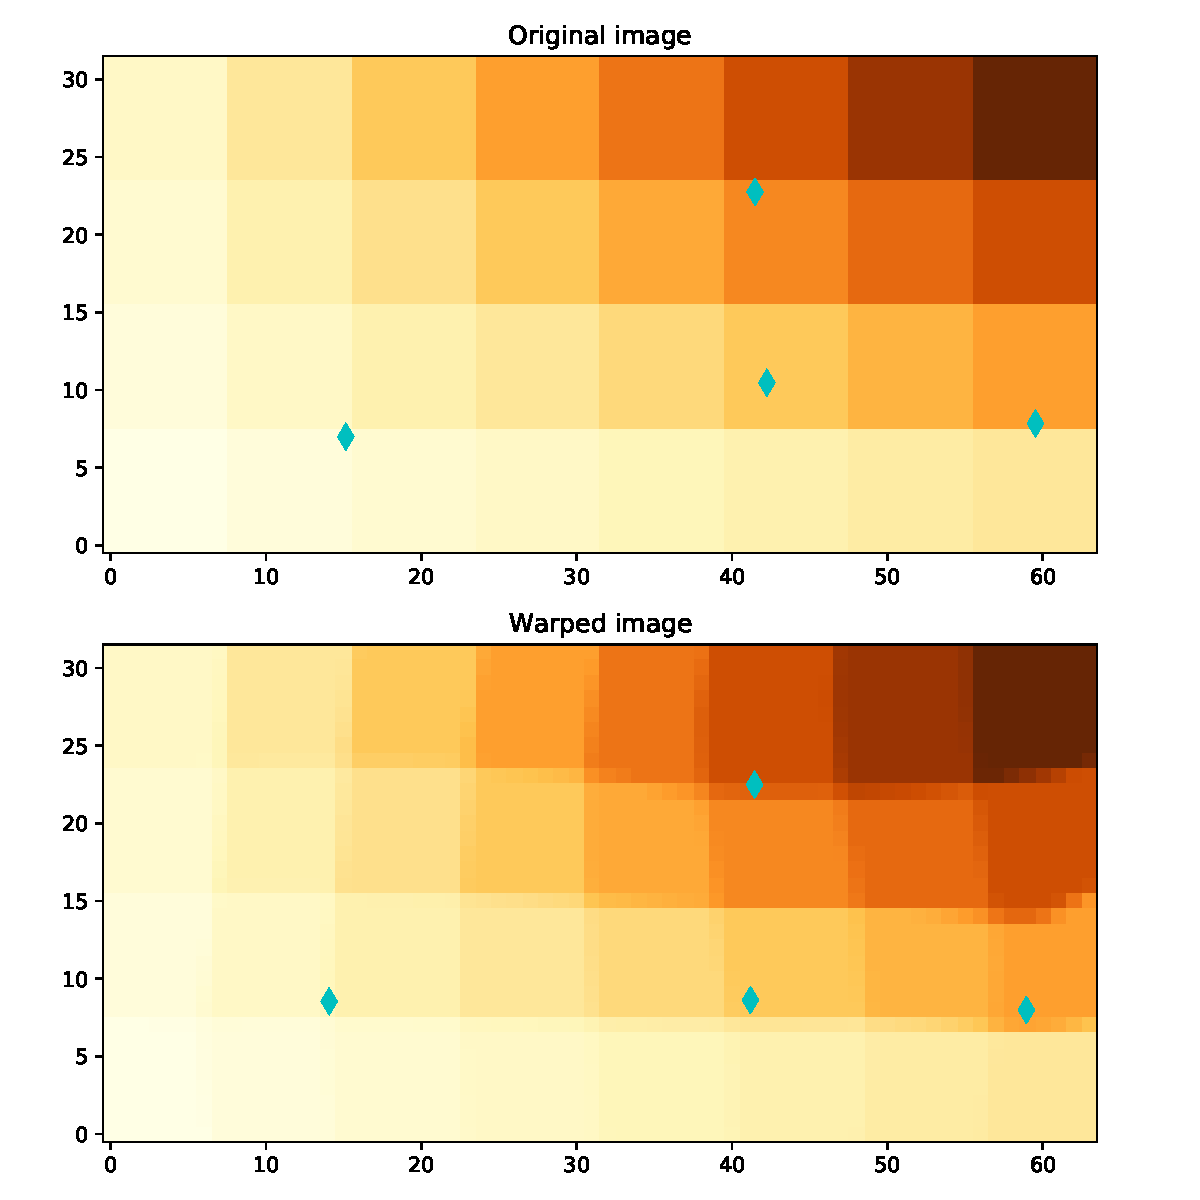
\includegraphics[width=0.8\linewidth]{warp_grid.pdf}
    \caption{
    The effects of \texttt{sparse\_image\_warp} on an image, with
\texttt{num\_landmarks} $=4$, \texttt{max\_warp\_time} $=2$ and
\texttt{max\_warp\_freq} $=2$. The diamonds show the source and destination
landmarks.}%
    \label{fig:warp_grid}
\end{figure}

\begin{table*}[t!]
    \centering
    \caption{Values used to augment the dataset. The first lines list the parameters used to compute the spectrograms.}
    \label{tab:aug_values}
    \begin{tabular}{|c|cccccc|}
        \hline
        & mel\_kwargs & n\_mel & n\_fft & hop\_length & fmin & fmax \\
        \hline
        & mel\_01 & 64 & 1024 & 256 & 40 & 8000  \\
        & mel\_02 & 128 & 2046 & 512 & 40 & 8000  \\
        & mel\_03 & 64 & 1024 & 256 & default & default  \\
        \hline
        \hline
        aug name & max\_time\_shifts & stretch\_rate & mel\_kwargs & num\_landmarks & max\_warp\_time & max\_warp\_freq\\
        \hline
        aug01 &  [1600, 3200] & [0.8, 1.2] & mel\_01 & 3 & 5 & 6 \\
        aug02 &  [] & [] & mel\_02 & 3 & 5 & 5 \\
        aug03 &  [] & [] & mel\_02 & 3 & 5 & 0 \\
        aug04 &  [] & [] & mel\_02 & 3 & 0 & 5 \\
        aug05 &  [] & [] & mel\_02 & 3 & 0 & 0 \\
        aug06 &  [] & [] & mel\_01 & 3 & 5 & 5 \\
        aug07 &  [] & [] & mel\_01 & 3 & 5 & 0 \\
        aug08 &  [] & [] & mel\_01 & 3 & 0 & 5 \\
        aug09 &  [] & [] & mel\_01 & 3 & 0 & 0 \\
        aug10 &  [] & [] & mel\_03 & 3 & 5 & 5 \\
        aug11 &  [] & [] & mel\_03 & 3 & 5 & 0 \\
        aug12 &  [] & [] & mel\_03 & 3 & 0 & 5 \\
        aug13 &  [] & [] & mel\_03 & 3 & 0 & 0 \\
        \hline
    \end{tabular}
\end{table*}

\section{Learning Framework}
\label{sec:learning_framework}

How did it learn anything at all?

\subsection{Learning rate schedule}

\subsubsection{Fixed LR}
\subsubsection{Exp decay LR}
\subsubsection{Cyclic LR}

\subsection{Hyper-parameter tuning}

\section{Convolutional Neural Network}
\label{sec:convolutional_arch}

\subsection{Architecture}

As a starting benchmark, a standard Convolutional Neural Network was implemented.
Three convolutional modules are instantiated, followed by a dense classifier.
Each convolutional module is composed of the convolutional layer, a batch
normalization layer, a max pooling layer and a dropout layer.
The classifier is composed by three dense layers, the last with softmax
activation and a number of units equal to the number of classes to predict.

\subsection{Model hyper-parameters}

When building the model, aside from the number of classes to predict and the
input shape of the spectrogram, five parameters can be set:

\begin{enumerate}
    \item Number of convolutional filters: deeper layers have to learn more
        filters, as the feature maps decrease in width and height after the
        pooling.
    \item Shape of the convolutional filters:
        both square and rectangular filters were tested.
        A vertical rectangular filters (e.g. (5, 1)) emphasizes the
        relationship between mel coefficients within the same time step
    \item Shape of the pooling window: 
        both square and rectangular windows were tested.
        Again, a rectangular filter allows to push into deeper layers more
        information along the time or frequency axis.
    \item Dropout rates after the convolutional modules.
    \item Width of the dense classifier layers.
\end{enumerate}

TODO: the hypa values

\section{Transfer Learning Approach}
\label{sec:transfer_learning}

\section{Attention Model}
\label{sec:attention_model}

\subsection{Attention architecture}

\subsection{Query style}

\subsection{AreaNet}

Dream a dream

